\documentclass[11pt,a4paper]{article}

% ============================================================
% JART MANUSCRIPT — PHASE 2
% ============================================================
\usepackage[
  paperwidth=21cm,
  paperheight=29.7cm,
  top=2.5cm,
  bottom=2.5cm,
  left=2.5cm,
  right=2.5cm
]{geometry}

% Compile with XeLaTeX or LuaLaTeX
\usepackage{fontspec}
\IfFontExistsTF{Times New Roman}
  {\setmainfont{Times New Roman}}
  {\setmainfont{TeX Gyre Termes}}

% Unicode text is supported directly through XeLaTeX + fontspec.

\usepackage{booktabs}
\usepackage{array}
\usepackage{tabularx}
\usepackage{longtable}
\usepackage{multirow}
\usepackage{amsmath}
\usepackage{amssymb}
\usepackage{graphicx}
\usepackage{caption}
\AtBeginDocument{%
  \renewcommand{\tablename}{Table}%
  \renewcommand{\figurename}{Figure}%
  \renewcommand{\refname}{References}%
}
% Shared bibliography for PDF and DOCX builds.
\usepackage[backend=biber,style=apa,natbib=true,sorting=nyt]{biblatex}
\addbibresource{references.bib}
\newcounter{journalbib}
\defbibenvironment{bibliography}
  {\list{\arabic{journalbib}.}{\usecounter{journalbib}\setlength{\leftmargin}{1.7em}\setlength{\labelwidth}{1.2em}\setlength{\labelsep}{.5em}\setlength{\itemsep}{4pt}}}
  {\endlist}{\item}
\usepackage{microtype}
\setlength{\emergencystretch}{2em}
\newcommand{\mbs}{\,\mathrm{MB/s}}
\usepackage[hidelinks]{hyperref}
\usepackage{xurl}
\urlstyle{same}
\usepackage{titlesec}
\usepackage{placeins}


% ============================================================
% STYLE SETTINGS
% ============================================================
\pagestyle{plain}
\linespread{1.0}
\setlength{\parindent}{0.5cm}
\setlength{\parskip}{0pt}

\captionsetup{
  font=small,
  labelfont=bf,
  textfont=it,
  labelsep=newline,
  justification=raggedright,
  singlelinecheck=false
}

\titleformat{\section}
  {\normalfont\fontsize{12}{14}\bfseries}
  {\thesection.}
  {0.5em}
  {}

\titleformat{\subsection}
  {\normalfont\fontsize{11}{13}\bfseries}
  {\thesubsection.}
  {0.5em}
  {}

\titleformat{\subsubsection}
  {\normalfont\fontsize{11}{13}\bfseries}
  {\thesubsubsection.}
  {0.5em}
  {}

\titlespacing*{\section}{0pt}{10pt}{6pt}
\titlespacing*{\subsection}{0pt}{8pt}{4pt}
\titlespacing*{\subsubsection}{0pt}{6pt}{3pt}

\graphicspath{{figures/}}
\renewcommand{\topfraction}{0.85}
\renewcommand{\textfraction}{0.1}
\renewcommand{\floatpagefraction}{0.85}
\AtBeginBibliography{\interlinepenalty=10000}
\hypersetup{pdftitle={Experimental Evaluation of CPU AES-NI and CUDA Encryption: Data Transfer Overhead and Cost-Efficiency Implications}}
\hypersetup{pdfauthor={Marko Mihajlović}}

\begin{document}
\begin{center}
{\fontsize{15}{18}\selectfont\bfseries Experimental Evaluation of CPU AES-NI and CUDA Encryption: Data Transfer Overhead and Cost-Efficiency Implications\par}
\medskip
{\bfseries Marko Mihajlović\par}
Faculty of Informatics and Computing\\
Singidunum University\\
Belgrade, Serbia\\
\href{mailto:marko.mihajlovic.23@singimail.rs}{marko.mihajlovic.23@singimail.rs}\\
ORCID: 0009-0006-7979-0341
\end{center}

\section*{Abstract}
This study evaluates how implementation choices, data location, and timing boundaries influence AES-128-CTR execution on heterogeneous CPU/GPU platforms. Five validated sessions on an Intel i5-10300H and NVIDIA GTX 1650 Ti compare a PyCryptodome AES-NI transform, a resident CUDA kernel, and a prepared transfer-inclusive pipeline. At 32 MiB, the respective throughputs are 1455.8, 4800.6, and 1204.5 decimal MB/s. The resident kernel achieves approximately 3.30 times the CPU throughput, whereas the pipeline remains slower than the CPU at 1, 16, and 32 MiB. Payload transfers, synchronization, and host overhead change the observed outcome; the difference is not a direct estimate of PCIe transfer time. A separate Linux/Tesla T4 campaign compares independent 1 MiB page batches against a prepared native OpenSSL EVP transform. Increasing the batch from one to 32 pages raises the median of five session CPU/GPU time ratios from 0.5404 to 0.9125, without a GPU pipeline crossover. A secondary resource-time model gives GPU-to-CPU hourly-charge thresholds of 0.9503, 0.7626, and 0.8273 for the GTX pipeline. Equal consistently attributed hourly charges favor the tested CPU path. The contribution is a validated, boundary-explicit evaluation supporting practical execution-path selection; the cost thresholds are conditional engineering indicators, not measured financial savings.

\noindent\textbf{Keywords:} AES-128-CTR; AES-NI; CUDA; GPU acceleration; heterogeneous computing; performance benchmarking; data transfer overhead; cost efficiency.

\section{Introduction}
Heterogeneous computing offers several ways to accelerate encryption: dedicated CPU instructions reduce the cost of AES rounds, while GPUs execute many independent blocks concurrently. AES specifies the block transformation, and counter mode (CTR) permits parallel encryption of counter blocks followed by combination with the plaintext \citep{nist_aes2023,nist_ctr2001}. These properties make AES-128-CTR a useful workload for examining the relationship between computational acceleration and data movement.

A GPU kernel can process device-resident data rapidly while providing little benefit when plaintext and ciphertext must cross the host--device boundary. The relevant execution path therefore depends on where data originate and where their output is consumed \citep{gregg2011}. Equally, a GPU compared only against an unoptimized CPU implementation can appear advantageous because of software choices rather than the relative capabilities of the processors \citep{lee2010}. AES-NI is an appropriate hardware-accelerated CPU reference because it exposes dedicated AES instructions through commonly used cryptographic libraries \citep{intel_aesni}. It does not, by itself, establish the maximum throughput of a multicore processor.

Accessible laptop and shared research platforms allow these questions to be investigated with inspectable code and repeatable workloads. Their value is methodological accessibility, rather than representativeness of every production server. Reproducibility requires correctness checks, recorded software versions, matched inputs, explicit timers, and preservation of session-level observations. It also requires negative results: a slower transfer-inclusive GPU path is relevant to execution-path selection even when the same device has higher kernel throughput.

The research question is: \emph{How do implementation choices, data location, and measurement boundaries influence the observed performance and conditional resource cost of AES-128-CTR encryption?} Using the existing validated measurements, this paper makes three contributions:
\begin{enumerate}
\item A validated experimental comparison of CPU AES-NI and CUDA execution paths on an i5-10300H/GTX 1650 Ti platform, separating compute-only and transfer-inclusive measurements and documenting their preparation and allocation policies.
\item An independent analysis of batched AES-128-CTR processing on Tesla T4, using a separately defined CPU OpenSSL EVP baseline and independent 1 MiB pages.
\item A conditional resource-cost decision model derived from measured throughput, with explicit charging assumptions, estimator distinctions, and limits on application-level interpretation.
\end{enumerate}
The first two contributions establish the technical evidence for the third. Separating transfer time from kernel execution is established practice, not a new research concept. The present study evaluates specific implementations and workloads; it does not propose a new cipher or a comprehensive economic or energy model.

\section{Related Work}
\subsection{GPU AES implementations and heterogeneous execution}
\citet{iwai2012} studied CUDA AES on a GeForce GTX285, examining the interaction of processing granularity and memory allocation. Their implementation also overlapped processing with data transfer and reported transfer-inclusive throughput. Thus, transfer-aware AES evaluation predates this study. Our comparison uses a different hardware/software pair, a verified AES-NI library path, and a synchronous prepared pipeline; it does not attempt to reproduce their optimized throughput.

\citet{tezcan2021} optimized GPU AES by addressing shared-memory bank conflicts and evaluated implementations on several GPU architectures. That work investigates kernel optimization and high computational throughput. Our byte-oriented CUDA baseline and modest loop-unrolling variant serve as inspectable experimental implementations, not as competitors for state-of-the-art kernel performance. Their role is to test how a validated implementation's observed advantage changes when the timed interval includes payload movement.

\citet{fei2020} studied parallel AES energy efficiency using a K20M GPU and two Xeon E5-2640 v2 processors. Their approach combines workload balancing, frequency adjustment, communication/computation overlap, and occupancy considerations. That energy-oriented hybrid execution differs from our separately timed CPU and GPU paths. We do not measure energy and therefore do not infer joules per GB from throughput or device power specifications.

\citet{yang2025} address AES encryption and decryption in CBC and CTR modes and propose a hybrid CPU/GPU workflow with performance evaluation and computational modeling. Their scope concerns hybrid workflow selection across hardware models. Here, the evidence is restricted to validated AES-128-CTR encryption records, explicitly defined prepared-workload boundaries, and separate campaign-level estimators; no hybrid scheduler or decryption performance is evaluated.

\subsection{Data location, fair baselines, and measurement scope}
\citet{gregg2011} demonstrate across GPU workloads that data location and required transfers determine whether kernel speed translates into useful acceleration. Their general CPU/GPU comparison framework motivates our separation of resident and host-memory paths. \citet{lee2010} show why optimizations appropriate to both architectures matter when reporting speedups. We apply that principle by selecting an explicit AES-NI path and by treating the later native EVP baseline as a different implementation, rather than substituting it into an earlier GPU campaign. Neither study supplies the AES-CTR measurements reported here.

The CUDA best-practices documentation distinguishes device-event timing from host timing and discusses pinned memory and asynchronous transfer/computation overlap \citep{nvidia_guide}. These mechanisms explain why preparation policy and synchronization must be reported. Our synchronous pipeline does not test an overlapped production implementation, and its event and wall-clock components are not an exact additive decomposition of bus and computation costs.

The specific contribution is therefore an audited comparison of three AES execution boundaries on accessible hardware, a separately analyzed independent-page batch workload with native EVP, and a conditional resource-charge interpretation of the measured results. This combines implementation validation and estimator-aware reporting without claiming that earlier research ignored transfers or hardware-accelerated CPU baselines.

\section{Methodology and Timing Boundaries}
\subsection{Primary platform and implementations}
The primary platform is a Windows 10 x64 machine (build 19045) with an Intel Core i5-10300H (four physical/eight logical cores), approximately 16 GB RAM, and an NVIDIA GTX 1650 Ti (4 GB class). The archived environment records Python 3.12.10, PyCryptodome 3.23.0, CuPy 13.6.0, CUDA runtime API version 12090, and driver API version 13030. These are recorded API versions, not inferred driver-package release numbers.

AES-128-CTR uses a 128-bit key and a full 128-bit big-endian counter in the primary campaign, with counter-space exhaustion rejected. The CPU factory explicitly requests the PyCryptodome AES-NI backend. An untimed native-initialization observer verifies the selected backend and saved capability checks; this is dispatch evidence, not instruction tracing. CPU performance is measured through a \emph{single-stream CPU AES-NI transform path with single-threaded application-level orchestration}, using one synchronous \texttt{encrypt()} call per observation. No physical-core pinning was established, and native thread execution was not independently traced. The measured rate is not aggregate multicore CPU capacity.

The CUDA baseline assigns one 16-byte AES block to each thread and launches 128 threads per CUDA block. Key expansion is a separate untimed operation. Variant v1 retains the byte-oriented AES rounds, S-box placement, counter semantics, and timing adapter, while adding explicit round/column loop unrolling and inlining. It does not add fused T-tables, shared-memory tuning, or asynchronous overlap. A separately tested T-table candidate did not enter the final timed dataset. Reporting both baseline and v1 avoids presenting a selected fastest kernel as representative of all CUDA AES implementations.

\subsection{Correctness, pairing, and repeated sessions}
Validation precedes timing. Saved known-answer and differential tests, counter-wrap rejection, native-backend checks, and output hashes passed in all five primary study sessions. Each measured output was compared with its reference after timing; a mismatch prevented acceptance. Every paired job used the same plaintext, key, and counter, confirmed by the stored input digest. Input generation and reference encryption were outside the measurement windows.

Five independent study sessions on the same hardware pair used seeds 2003--2007, five warm-up iterations, and twenty retained repetitions per configuration. They are independent process runs, not five independent machines. Within each repetition, mode and backend/scope job order were seed-shuffled, while input sizes followed the configured ascending order. The broader ECB/CTR campaign contains 6000 retained observations across five sizes (1 KiB, 16 KiB, 1 MiB, 16 MiB, and 32 MiB); this paper focuses on the three large CTR sizes relevant to its buffer-processing question. Smaller sizes remain in the audit, where launch/copy overhead further limits GPU pipeline performance. Historical warm-ups are documented by source and configuration but were not exported as retained rows. No retained samples were removed.

\subsection{Measured intervals and excluded operations}
Figure~\ref{fig:boundaries} illustrates the three primary timing boundaries. CPU wall time brackets the synchronous encryption call, including output allocation and Python/native-call overhead, but excludes cipher construction and key scheduling. The GPU resident result is a CUDA-event interval around one kernel launch after payload upload. Completion is awaited before reading the event duration; the host waiting time is not separately added to that device-event metric. Payload download and validation occur afterward.

\begin{figure}[htbp]
\centering
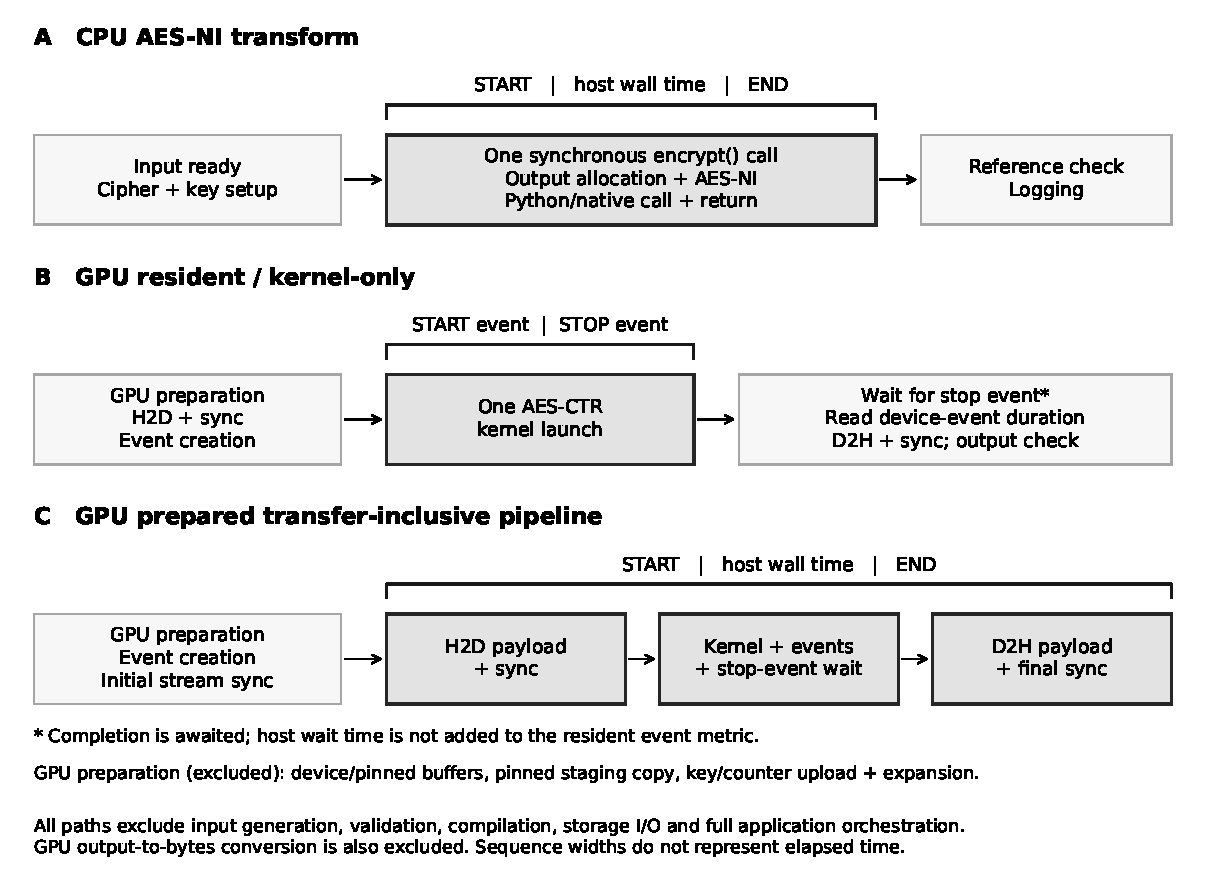
\includegraphics[width=\linewidth]{measurement_boundaries.pdf}
\caption{Primary GTX campaign measurement boundaries, reconstructed from the archived timing adapter. Dark outlines mark the measured intervals; pale boxes are excluded preparation or follow-up operations. H2D and D2H denote host-to-device and device-to-host payload transfers. Sync denotes completion synchronization. Sequence widths are schematic, not measured durations.}
\label{fig:boundaries}
\end{figure}

The prepared GPU pipeline uses host wall time from H2D submission through completed D2H transfer and synchronization. It includes synchronization after H2D, kernel event recording and launch, the kernel completion wait, D2H, and final synchronization. Initial stream synchronization and event creation precede the timer. Device and pinned-host buffer allocation, copying plaintext into the pinned buffer, key/counter upload and expansion, compilation, and output-to-bytes conversion are excluded. CPU input is an ordinary bytes object; GPU input has already been staged in pinned memory.

Consequently, the CPU and pipeline comparisons begin and end with host data at a broad functional level, but differ in allocation and wrapper overhead. They are prepared in-memory path comparisons, not a complete application-level end-to-end benchmark. Neither path includes storage I/O, networking, authentication, scheduling queues, or an application protocol. This distinction matters even when both output ciphertexts are identical.

\subsection{Aggregation and estimators}
For a payload of $N$ bytes and measured duration $T$ seconds, throughput in decimal MB/s is
\begin{equation}\label{eq:rate}
R=\frac{N}{10^6T}.
\end{equation}
Payload sizes in MiB use $2^{20}$ bytes. Let $r_{j,s,k}$ and $T_{j,s,k}$ denote rate and time for path $j$, session $s$, and retained repetition $k$. The reported aggregate rate and paired CPU/GPU time ratio are
\begin{equation}\label{eq:estimators}
\widehat R_j=\operatorname{median}_{s=1}^{5}\operatorname{median}_{k=1}^{20}r_{j,s,k},
\qquad
\widehat q=\operatorname{median}_{s=1}^{5}
\frac{\operatorname{median}_{k}T_{C,s,k}}{\operatorname{median}_{k}T_{G,s,k}}.
\end{equation}
The ratio $\widehat R_G/\widehat R_C$ need not equal $\widehat q$. Even within a session, a median of twenty reciprocal times need not equal the reciprocal of the median time because the two central observations are averaged. Session medians are the aggregation units; the one hundred retained repetitions per configuration are not pooled as one hundred independent study sessions. Reported session ranges describe observed variation, not confidence intervals.

\subsection{Separate Tesla T4 independent-page campaign}
The T4 study uses a Linux x86-64 research environment with an Intel Xeon host reported at 2.00 GHz and two visible logical CPUs, and a Tesla T4 (compute capability 7.5; approximately 15.6 billion reported device-memory bytes). Saved metadata records Linux 6.6.159+, Python 3.13.16, CuPy 14.0.1, CUDA runtime and driver API version 13000, and OpenSSL 3.0.13 with its default provider. CPU AES capability is recorded; executed instructions were not traced. This native EVP path is distinct from the Windows/PyCryptodome AES-NI path.

Batches contain 1, 4, 16, or 32 independent 1 MiB pages. Each page uses a distinct structured 96-bit nonce and a 32-bit counter beginning at one; duplicate nonces and counter overflow are rejected. Deterministic test material reproduces logical messages across paths and is not a production nonce-generation policy. One GPU launch maps AES blocks to pages and within-page counters, retaining the original AES rounds. The CPU uses one sequential native loop over preinitialized EVP contexts. Its transformation timer includes EVP Update/Final calls, loop overhead, and length checks, but excludes output allocation, context initialization, FFI, cleanup, and output conversion. The GPU prepared pipeline inherits the primary adapter's transfer-inclusive interval; nonce-table preparation/upload is also excluded.

Five sessions with seeds 2003--2007 again use five warm-ups and twenty retained repetitions. Batch and job orders are shuffled. Saved pre-timing validation covers 25 cases, including published vectors, partial blocks, page boundaries, and counter carries; timed outputs are checked outside the timer. Warm-up rows are preserved but excluded from statistics. For each batch size, the CPU-transform/GPU-pipeline ratio is computed from session median times, then summarized by its median across five sessions as in Equation~\eqref{eq:estimators}. Different CPU implementations, operating systems, allocation policies, and counter/message layouts preclude pooling with the GTX campaign.

\subsection{Evidence provenance and reproducibility}
This revision analyzes existing records; it adds no benchmarks. The primary records are the five September 30, 2026 paired-study directories, and the page records are the five archived \texttt{t4-phase2-study} sessions. The accompanying analysis directory \texttt{economic\_aes\_existing\_evidence\_2026\_10} contains reconstructed session/aggregate results, source and input hashes, threading and boundary audits, and conditional cost indicators. Saved validation flags, complete retained grids, paired hashes, and archived source identities were checked by that audit. The Phase 1 reproduction scripts read those records without running encryption and regenerate the reported figures and numerical checks. These files support local reproducibility; a public raw-data archive is not assumed merely because source code is available.

\section{Results}
\subsection{Primary CPU and CUDA throughput}
Table~\ref{tab:primary} retains the audited aggregate throughputs for the CPU and both CUDA variants. Figure~\ref{fig:throughput} presents the baseline comparison. The resident GPU kernel is faster than the tested CPU transform at all three sizes, whereas both prepared GPU pipelines remain slower than that CPU path.

\begin{table}[htbp]\centering\small
\caption{AES-128-CTR throughput on GTX 1650 Ti / i5-10300H, decimal MB/s; five sessions. K: resident kernel; P: prepared pipeline.}\label{tab:primary}
\setlength{\tabcolsep}{4pt}
\begin{tabular}{lrrrrr}\toprule
Input & CPU AES-NI & CUDA K & CUDA P & v1 K & v1 P\\\midrule
1 MiB & 1381.7 & 5017.1 & 1313.1 & 4853.9 & 1291.0\\
16 MiB & 1446.5 & 3655.6 & 1103.1 & 3576.2 & 1074.0\\
32 MiB & 1455.8 & 4800.6 & 1204.5 & 4877.7 & 1209.1\\\bottomrule
\end{tabular}
\end{table}

\begin{figure}[htbp]
\centering
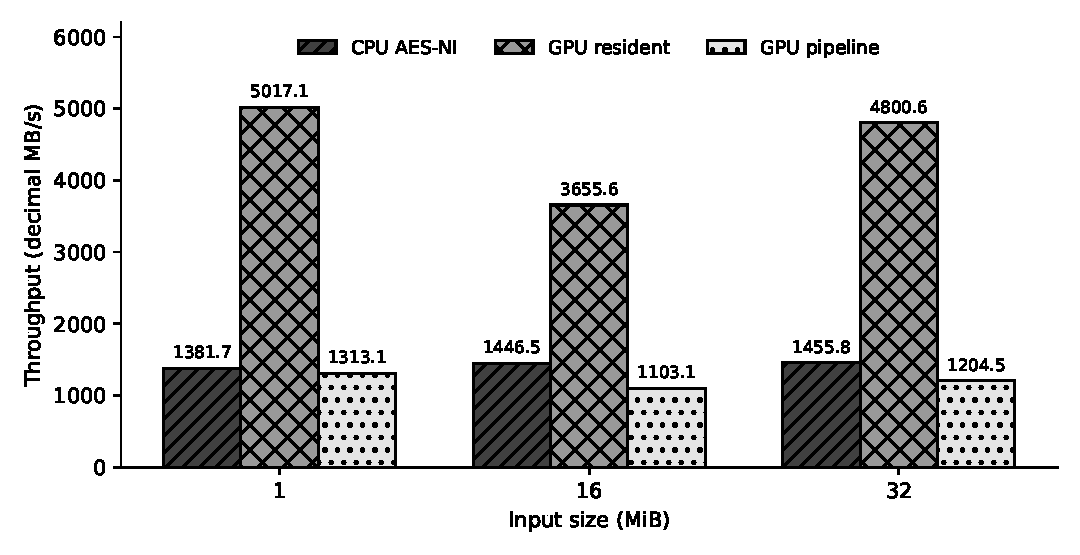
\includegraphics[width=\linewidth]{aes_throughput_comparison.pdf}
\caption{Measured throughput of AES-128-CTR execution paths on i5-10300H/GTX 1650 Ti: CPU AES-NI, resident GPU kernel, and prepared GPU pipeline. Decimal MB/s; median of five session medians.}
\label{fig:throughput}
\end{figure}

At 32 MiB, the baseline resident kernel achieves 4800.6 MB/s versus 1455.8 MB/s for CPU AES-NI, approximately 3.30 times the throughput. Adding the prepared transfer-inclusive boundary changes the GPU result to 1204.5 MB/s, below the CPU. The separately calculated median of session CPU/GPU time ratios is 0.8233 for the pipeline (session range 0.8217--0.8422); it is not the aggregate-rate ratio of 0.8273. At 1 and 16 MiB, the paired pipeline ratios are 0.9529 and 0.7496, respectively, and every session favors the tested CPU transform.

The gap between resident and pipeline performance demonstrates the consequence of changing the measured interval, not an isolated estimate of PCIe transfer cost. The pipeline includes transfers, synchronization, and host launch/event overhead, and resident and pipeline timings come from separate executions. Even the pipeline's own device-event component and host-clock intervals use different clocks; subtracting them does not provide a pure bus-time measurement.

The GPU throughput dip at 16 MiB is retained. Its paired pipeline ratio ranges from 0.5619 to 0.7668 across sessions, wider than at 32 MiB. No causal explanation was isolated: fixed size order, dynamic clocks, operating-system scheduling, and memory behavior were not independently varied. The data therefore do not support a monotonic scaling law. Variant v1 also shows no consistent improvement: its resident/pipeline rates are lower than baseline at 1 and 16 MiB and slightly higher at 32 MiB. Explicit unrolling alone does not establish production-level optimization.

\subsection{Independent-page batching on Tesla T4}
Figure~\ref{fig:t4pages} retains the independently audited T4 results. The medians of session-level CPU EVP transform/GPU pipeline time ratios are 0.5404, 0.7137, 0.8240, and 0.9125 for 1, 4, 16, and 32 pages. Every ratio remains below one in all five sessions. Larger batches narrow the relative pipeline gap over the tested grid, but do not establish a GPU crossover.

\begin{figure}[htbp]
\centering
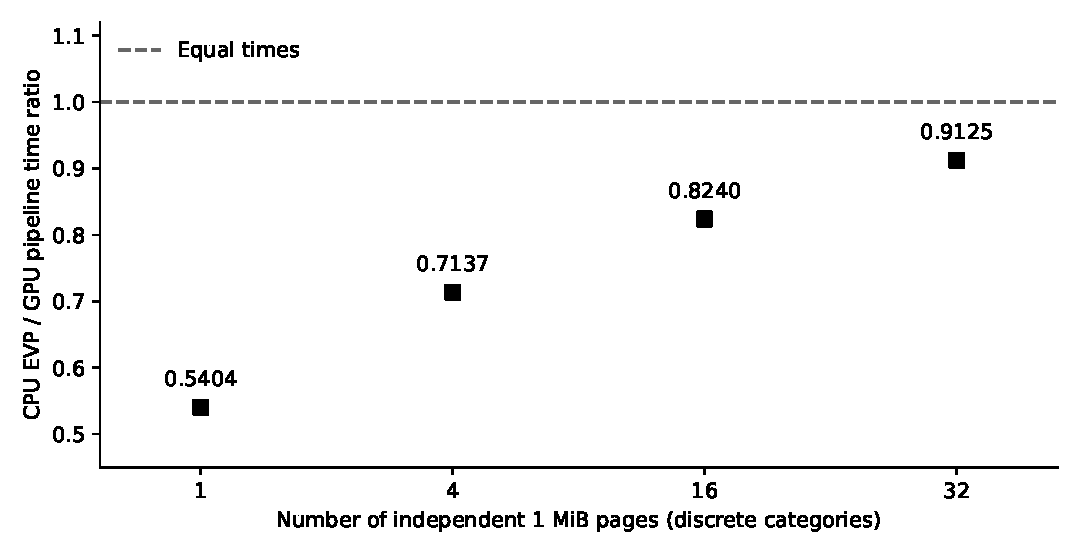
\includegraphics[width=.90\linewidth]{t4_page_batch_ratios.pdf}
\caption{Separate Linux/T4 study of independent AES-128-CTR pages (1 MiB per page): median of five ratios of session median CPU EVP transform time to prepared GPU pipeline time. Values below 1 favor the CPU; the horizontal line denotes equal times. Batch sizes are discrete categories; this is not a direct comparison of T4 and GTX results.}
\label{fig:t4pages}
\end{figure}

At 32 pages, 0.9125 corresponds to approximately 8.75\% shorter CPU time relative to GPU time under this estimator. This percentage is derived from paired session ratios, not from pooled observations or division of separately aggregated rates. Batching changes the amount of work submitted per launch and the CPU's sequential page loop; the observed trend is consistent with amortizing fixed overhead but does not isolate a single cause. No crossing point is extrapolated beyond 32 pages. These measurements characterize synthetic independent pages, not an implemented Parquet reader or writer.

\section{Conditional Cost-Efficiency Implications}
Let $h_C$ and $h_G$ be consistently attributed hourly resource charges for the CPU and GPU execution paths, with $h_G$ including the required host resources. For repeated processing at aggregate rate $\widehat R_j$, the modeled duration per decimal GB and resource-time cost are
\begin{equation}\label{eq:cost}
t_j=\frac{1000}{\widehat R_j},\qquad c_j=\frac{h_jt_j}{3600}.
\end{equation}
Seconds per GB are derived by repeating the observed batch rate; a contiguous 1 GB request or sustained service was not measured. The model assumes proportional occupied-time charging, comparable accounting periods, and consistently attributed capacity. It excludes minimum billing increments, queueing, idle reservations, and utilization adjustments. For positive charges, $c_G<c_C$ when
\begin{equation}\label{eq:threshold}
\frac{h_G}{h_C}<\frac{\widehat R_G}{\widehat R_C}.
\end{equation}
Throughput is empirical; the time-per-GB values and charge thresholds are derived; hourly charges are assumed. Actual financial costs were not measured.

Table~\ref{tab:econ} reports the baseline GTX pipeline thresholds using unrounded aggregate rates. Setting each hourly charge to one normalized unit gives a transparent equal-charge comparison, not a currency price.

\begin{table}[htbp]\centering\small
\caption{Conditional resource-time cost indicators for CPU AES-NI and the CUDA baseline pipeline. Costs are normalized units/GB, not market currencies.}\label{tab:econ}
\begin{tabular}{lrrr}\toprule
Input & $R_G/R_C$ & $c_C$ ($h_C=1$) & $c_G$ ($h_G=1$)\\\midrule
1 MiB & 0.9503 & 0.0002010 & 0.0002116\\
16 MiB & 0.7626 & 0.0001920 & 0.0002518\\
32 MiB & 0.8273 & 0.0001908 & 0.0002306\\\bottomrule
\end{tabular}
\end{table}

At equal consistently attributed hourly charges, the tested CPU AES-NI path has lower modeled cost for these host-memory workloads. At 32 MiB, the pipeline requires a GPU-to-CPU charge ratio below 0.8273, or about 82.73\%, to reverse that decision under the aggregate-rate model. This is a relative service-charge condition, not a purchase-price discount or measured saving. One CPU core's charge cannot be compared with a whole GPU server's charge without a consistent allocation of capacity to the task.

The retained sensitivity grid assumes $h_C=1$ and $h_G/h_C\in\{0.50,0.75,1.00,1.25,1.50,2.00\}$. The aggregate-rate model favors the pipeline at 0.50 and 0.75 and the CPU at the higher ratios for these sizes. The 16 MiB result at 0.75 is borderline: its paired-time threshold median is 0.7496 and sessions vary. This illustrates why the choice of estimator and observed session variability matter near a decision boundary. Resident processing offers computational potential when transfers are unnecessary, but practical usefulness depends on the surrounding data-resident workflow, implementation, utilization, and resource prices. The model measures neither electricity savings nor TCO or return on investment.

\section{Discussion, Limitations, and Future Work}
\subsection{Execution-path selection and implementation effects}
The tested AES-NI path provides an effective hardware-accelerated reference for host-memory buffers. Its advantage over the synchronous CUDA pipelines shows why kernel-only speedup is insufficient for selecting an offload path. Conversely, the resident result identifies a plausible opportunity when encryption is embedded in a device-resident workflow. Whether that opportunity survives input preparation, subsequent computation, and output delivery remains an application-level question.

The byte-oriented CUDA baseline and v1 are experimental implementations. Optimized kernels, more favorable memory organization, and overlapped transfers could alter their performance, as the related work demonstrates. Likewise, a preallocated native EVP path has different overhead from an allocating PyCryptodome call. The T4 experiment deliberately uses the former within its own campaign; it cannot isolate an architectural GTX/T4 effect because host CPU, libraries, operating system, message layout, and timing policies also change. Shared execution environments and dynamic system state further limit hardware-wide conclusions.

The single-stream CPU measurement does not exhaust available multicore capacity. A multiworker AES-NI implementation could change aggregate throughput, memory contention, and attributable resource use, but those outcomes are not measured here. The result is an execution-path comparison within declared boundaries rather than a universal CPU/GPU capacity ranking.

\subsection{Independent pages, Parquet, and security}
Apache Parquet modular encryption provides a concrete use case for independent encrypted pages. Its \texttt{AES\_GCM\_CTR\_V1} mode uses CTR for pages and GCM for other modules, with a 96-bit nonce and 32-bit initial counter for CTR \citep{parquet_encrypt}. Our T4 workload borrows this page-level counter structure but does not implement Parquet framing, compression, metadata protection, storage I/O, key management, or its nonce-generation requirements. It therefore establishes neither Parquet acceleration nor GPU economic benefit for Parquet.

CTR supplies confidentiality without authentication and requires non-repeating counter blocks under a key \citep{nist_ctr2001}. Correct ciphertext on test vectors does not establish side-channel resistance or a secure deployment. Authentication and tamper detection require additional mechanisms; GCM incorporates an authentication component not measured in these CTR intervals \citep{nist_gcm2007}. Timing results cannot be transferred directly to a complete authenticated-encryption service.

\subsection{Limits and next steps}
Five repeated sessions support within-campaign comparisons, not population estimates for all processors. No controlled core affinity, causal diagnosis of the 16 MiB dip, sustained concurrent service, integrated energy measurement, or real resource-price dataset is available. Hardware accessibility makes repetition feasible but does not guarantee identical cloud capacity or operational cost. The conditional model is useful only after matching the chosen execution boundary to the resource attribution and data-location assumptions.

Realistic extensions are optimized CUDA kernels with transfer overlap, encryption within GPU-resident workflows, multiworker AES-NI baselines, and application-level Parquet processing. Energy instrumentation and documented resource prices would support additional engineering decisions. These are future investigations, not completed experiments in this paper.

\FloatBarrier
\section{Conclusion}
The existing validated AES-128-CTR measurements distinguish CPU transform throughput, resident CUDA computation, and a prepared transfer-inclusive pipeline. On the i5-10300H/GTX 1650 Ti platform, the resident kernel reaches 4800.6 MB/s at 32 MiB, approximately 3.30 times the CPU's 1455.8 MB/s, but the pipeline reaches only 1204.5 MB/s. The tested CPU AES-NI path is faster than the pipeline at all three reported sizes. Payload movement and the additional synchronization and host operations change the outcome; the difference cannot be assigned exclusively to PCIe transfer time.

The separate Tesla T4 study shows that increasing independent-page batches from one to 32 pages raises the median session CPU/GPU time ratio from 0.5404 to 0.9125. Batching narrows the pipeline's relative gap, but the prepared native EVP transform remains faster throughout the observed grid. This finding applies to its own software and measurement boundaries and supplies no extrapolated crossover.

The conditional cost model translates these technical results into explicit execution-path criteria. The GTX pipeline charge thresholds of 0.9503, 0.7626, and 0.8273 imply lower modeled CPU cost at equal consistently attributed hourly charges. They are useful for assessing a defined workload and resource-allocation scenario, not evidence of realized monetary or energy savings. Together, the experiments support boundary-aware path selection while limiting generalization to the tested implementations, data locations, and workloads.

\section*{Funding}
The author received no specific funding for this work.

\section*{Conflict of interest}
The author has no conflict of interest to declare.

\begingroup\fontsize{10}{12}\selectfont\sloppy
\printbibliography[title={References}]
\endgroup
\end{document}
